\documentclass[preprint,12pt]{elsarticle}

\usepackage{acronym}
\usepackage{array}
\usepackage{booktabs}
\usepackage{float}
\usepackage{graphicx}
\usepackage[section]{placeins}
\usepackage{tabularx}

\acrodef{bm}[BM25]{Best Matching 25}
\acrodef{ci}[CI]{confidence interval}
\acrodef{fn}[FN]{false negative}
\acrodef{fnr}[FNR]{false-negative rate}
\acrodef{fp}[FP]{false positive}
\acrodef{fpr}[FPR]{false-positive rate}
\acrodef{microns}[MICRONS]{Machine Intelligence from Cortical Networks}
\acrodef{svd}[SVD]{singular value decomposition}
\acrodef{tn}[TN]{true negative}
\acrodef{tp}[TP]{true positive}
\acrodef{vbn}[VBN]{Visual Behavior Neuropixels}
\acrodef{vv}[V\&V]{Verification and Validation}

\newcolumntype{Y}{>{\raggedright\arraybackslash}X}
\setlength{\emergencystretch}{2em}

% Preserve section order in the standalone supplement even though the shared
% table and figure sources use top-of-page placement in the main manuscript.
\let\standardtable\table
\let\endstandardtable\endtable
\renewenvironment{table}[1][]{\standardtable[H]}{\endstandardtable}
\let\standardfigure\figure
\let\endstandardfigure\endfigure
\renewenvironment{figure}[1][]{\standardfigure[H]}{\endstandardfigure}

\begin{document}

\begin{frontmatter}
\title{Supplementary Material for MouseClaimBench: Evidence-Constrained Knowledge-Based Reasoning for Mouse-Brain Claims}
\author[urjc]{Alberto Fern\'andez-Isabel}
\author[urjc]{Isaac Mart\'in de Diego}
\author[ucm]{Rub\'en Fuentes-Fern\'andez}
\affiliation[urjc]{organization={Rey Juan Carlos University},country={Spain}}
\affiliation[ucm]{organization={Complutense University of Madrid},country={Spain}}
\end{frontmatter}
\clearpage

\section{Methodological Comparison}

Table~\ref{tab:related-work-comparison} expands the comparison between MouseClaimBench and the closest methodological families summarized in the main paper.

\begin{table}[t!]
\centering
\caption{Relationship between MouseClaimBench and the closest methodological families. ``Partial'' indicates that the capability is present for a narrower objective than manuscript-level scientific claim authorization.}
\label{tab:related-work-comparison}
\footnotesize
\renewcommand{\arraystretch}{1.18}
\begin{tabularx}{\textwidth}{@{}p{0.22\textwidth}p{0.18\textwidth}p{0.13\textwidth}p{0.12\textwidth}Y@{}}
\toprule
Approach family & Decision object & Evidence binding & Veto rule & Manuscript action \\
\midrule
\ac{vv} and \ac{uq} & Model credibility for a context of use & Partial & Partial & No \\
Assurance cases & Structured claim and argument & Partial & Possible & Partial \\
Scientific claim verification & Textual support or refutation & Partial & No & Partial \\
Reproducibility and model reporting & Availability, execution, and declared limitations & Yes & No & No \\
MouseClaimBench & Admissible scientific wording & Yes & Yes & Yes \\
\bottomrule
\end{tabularx}
\end{table}


\section{Extended Experimental Design}

The main paper retains the protocol and all conclusions required to evaluate the contribution. Table~\ref{tab:experiment-design} provides the complete question-to-evidence map. Table~\ref{tab:oracle-policy-comparison} provides the oracle confusion counts and case-cluster intervals reported in the main text.

\begin{table}[t!]
\centering
\caption{Evaluation questions, evidence units, and maximum interpretations. The final column prevents software conformance from being reported as biological validation.}
\label{tab:experiment-design}
\footnotesize
\renewcommand{\arraystretch}{1.12}
\begin{tabularx}{\textwidth}{@{}p{0.07\textwidth}p{0.25\textwidth}p{0.29\textwidth}Y@{}}
\toprule
ID & Question & Evidence unit & Maximum admissible interpretation \\
\midrule
E1 & Is inference total, deterministic, and non-compensatory? & Profile validation and all 625 mechanistic state assignments & Rule-system correctness for the tested profile \\
\addlinespace[2pt]
E2 & Does the policy reduce unsupported authorization under known truth? & 500 structural-equation cases and 5,000 decisions per policy & Finite-sample comparison on five generated regimes \\
\addlinespace[2pt]
E3 & Does the KBS preserve the conclusions of real mouse artifacts? & Four cases, 40 frozen decisions, and 40 proof traces & Artifact-grounded conformance and bounded case interpretation \\
\addlinespace[2pt]
E4 & Can retrieval or association substitute for stronger evidence? & SciFact train/development claims and 108 Tuebingen pairs & External failure-mode control, not task state of the art \\
\addlinespace[2pt]
E5 & Are components and release artifacts internally consistent? & Legacy ablations, sensitivity grid, eight artifact families, revisions, and profile hash & Reproducible KBS method package with declared boundaries \\
\bottomrule
\end{tabularx}
\end{table}

\begin{table}[t!]
\centering
\caption{Oracle structural-equation benchmark over 500 generated cases and
5,000 claim decisions per policy. Intervals are 95\% Wilson intervals. \acs{fpr} and
\acs{fnr} retain their standard meanings and are not proposed as new metrics.}
\label{tab:oracle-policy-comparison}
\small
\renewcommand{\arraystretch}{1.13}
\begin{tabularx}{\textwidth}{@{}p{0.24\textwidth}rrrrYY@{}}
\toprule
Policy & \acs{tp} & \acs{fp} & \acs{tn} & \acs{fn} & \acs{fpr} (95\% \acs{ci}) & \acs{fnr} (95\% \acs{ci}) \\
\midrule
Evidence contract v3 & 1,954 & 56 & 2,844 & 146 & 0.019 (0.015--0.025) & 0.070 (0.059--0.081) \\
Prediction shortcut & 2,085 & 785 & 2,115 & 15 & 0.271 (0.255--0.287) & 0.007 (0.004--0.012) \\
\bottomrule
\end{tabularx}
\end{table}

\begin{table}[t!]
\centering
\caption{Oracle results by claim. Positive cases are defined by the generating
graph and intervention. Rates equal zero when a claim has no positive or
negative reference instances, so those rows are coverage checks rather than
performance estimates.}
\label{tab:oracle-claim-breakdown}
\footnotesize
\renewcommand{\arraystretch}{1.04}
\begin{tabularx}{\textwidth}{@{}Y r rr rr rr@{}}
\toprule
& & \multicolumn{2}{c}{Knowledge policy} & \multicolumn{2}{c}{Additive 0.75} & \multicolumn{2}{c}{Prediction shortcut} \\
\cmidrule(lr){3-4}\cmidrule(lr){5-6}\cmidrule(l){7-8}
Claim & Pos. & \acs{fpr} & \acs{fnr} & \acs{fpr} & \acs{fnr} & \acs{fpr} & \acs{fnr} \\
\midrule
Predictive & 400 & 0.000 & 0.013 & 0.000 & 0.013 & 0.000 & 0.013 \\
Computationally reproducible & 500 & 0.000 & 0.000 & 0.000 & 0.000 & 0.000 & 0.000 \\
Internally reproduced & 400 & 0.000 & 0.043 & 0.000 & 0.043 & 0.000 & 0.013 \\
Externally replicated & 0 & 0.000 & 0.000 & 0.000 & 0.000 & 0.000 & 0.000 \\
Topology specific & 300 & 0.000 & 0.020 & 0.000 & 0.020 & 0.500 & 0.017 \\
Directed & 200 & 0.153 & 0.295 & 0.153 & 0.295 & 0.650 & 0.000 \\
Local structure--function & 0 & 0.000 & 0.000 & 0.000 & 0.000 & 0.000 & 0.000 \\
Mechanistic & 200 & 0.033 & 0.295 & 0.333 & 0.000 & 0.650 & 0.000 \\
Causal & 100 & 0.000 & 0.000 & 0.000 & 0.000 & 0.738 & 0.000 \\
Complete entity-specific twin & 0 & 0.000 & 0.000 & 0.000 & 0.000 & 0.000 & 0.000 \\
\bottomrule
\end{tabularx}
\end{table}

\begin{table}[t!]
\centering
\caption{Oracle error rates by generating regime. Each row aggregates 100 cases while preserving the regime-specific prevalence of the ten claims.}
\label{tab:oracle-regime-breakdown}
\footnotesize
\renewcommand{\arraystretch}{1.08}
\begin{tabularx}{\textwidth}{@{}Y rr rr rr@{}}
\toprule
& \multicolumn{2}{c}{Knowledge policy} & \multicolumn{2}{c}{Additive 0.75} & \multicolumn{2}{c}{Prediction shortcut} \\
\cmidrule(lr){2-3}\cmidrule(lr){4-5}\cmidrule(l){6-7}
Regime & \acs{fpr} & \acs{fnr} & \acs{fpr} & \acs{fnr} & \acs{fpr} & \acs{fnr} \\
\midrule
Independent & 0.019 & 0.000 & 0.019 & 0.000 & 0.000 & 0.000 \\
Common cause & 0.023 & 0.000 & 0.046 & 0.000 & 0.571 & 0.000 \\
$X\rightarrow Y$ & 0.000 & 0.103 & 0.000 & 0.052 & 0.250 & 0.000 \\
$Y\rightarrow X$ & 0.038 & 0.070 & 0.162 & 0.070 & 0.475 & 0.038 \\
$X\rightarrow Y$ with intervention & 0.000 & 0.080 & 0.000 & 0.040 & 0.000 & 0.000 \\
\bottomrule
\end{tabularx}
\end{table}


\section{Artifact-Grounded Mouse-Brain Evidence}

Table~\ref{tab:real-case-summary} retains the original-scale observations, supported claims, and decisive limitation for each real case summarized in the main paper.

\begin{table}[t!]
\centering
\caption{Decisive observations and bounded claims in the four mouse-brain cases.}
\label{tab:real-case-summary}
\footnotesize
\renewcommand{\arraystretch}{1.02}
\begin{tabularx}{\textwidth}{@{}p{0.16\textwidth}p{0.39\textwidth}p{0.20\textwidth}Y@{}}
\toprule
Case & Observed rule and result & Supported claims & Decisive boundary \\
\midrule
Allen \acs{vbn} & Within-resource reproduction passes. Allen-minus-permutation is $-0.0054$, the bootstrap lower bound is $-0.0075$, and only $0.21$ of permutations are outperformed. All direction criteria equal zero. & Compute reproducibility and within-resource reproduction & Mechanistic claim blocked \\
\addlinespace[2pt]
Static Sensorium & Median best correlation is 0.341. Improvements over mean and scrambled baselines are 0.095 and 0.068. Topography passes in 5/5 datasets. & Prediction, within-resource reproduction, and topology specificity & No direction, intervention, or external replication \\
\addlinespace[2pt]
Dynamic Sensorium & Temporal \acs{svd} beats mean response in 4/5 and 5/5 mice. Median paired gains are 0.039 and 0.031. & Prediction and within-resource reproduction & Reliability is not estimable and temporal prediction is not biological direction \\
\addlinespace[2pt]
\acs{microns} local & The fixed endpoint passes in discovery and two hold-outs. Distance-matched deltas are 0.0215, 0.0210, and 0.0179. All unit-cluster interval lower bounds are positive. & Compute reproducibility, within-resource reproduction, and local observational structure--function association & One volume, observational endpoint, and no whole-brain coverage \\
\bottomrule
\end{tabularx}
\end{table}


\section{External Failure Controls}

SciFact tests whether retrieval or lexical support can replace claim authorization. Tuebingen tests whether association can replace causal direction. These experiments are failure-mode controls rather than competitive evaluations of the source tasks.

\begin{figure}[t!]
\centering
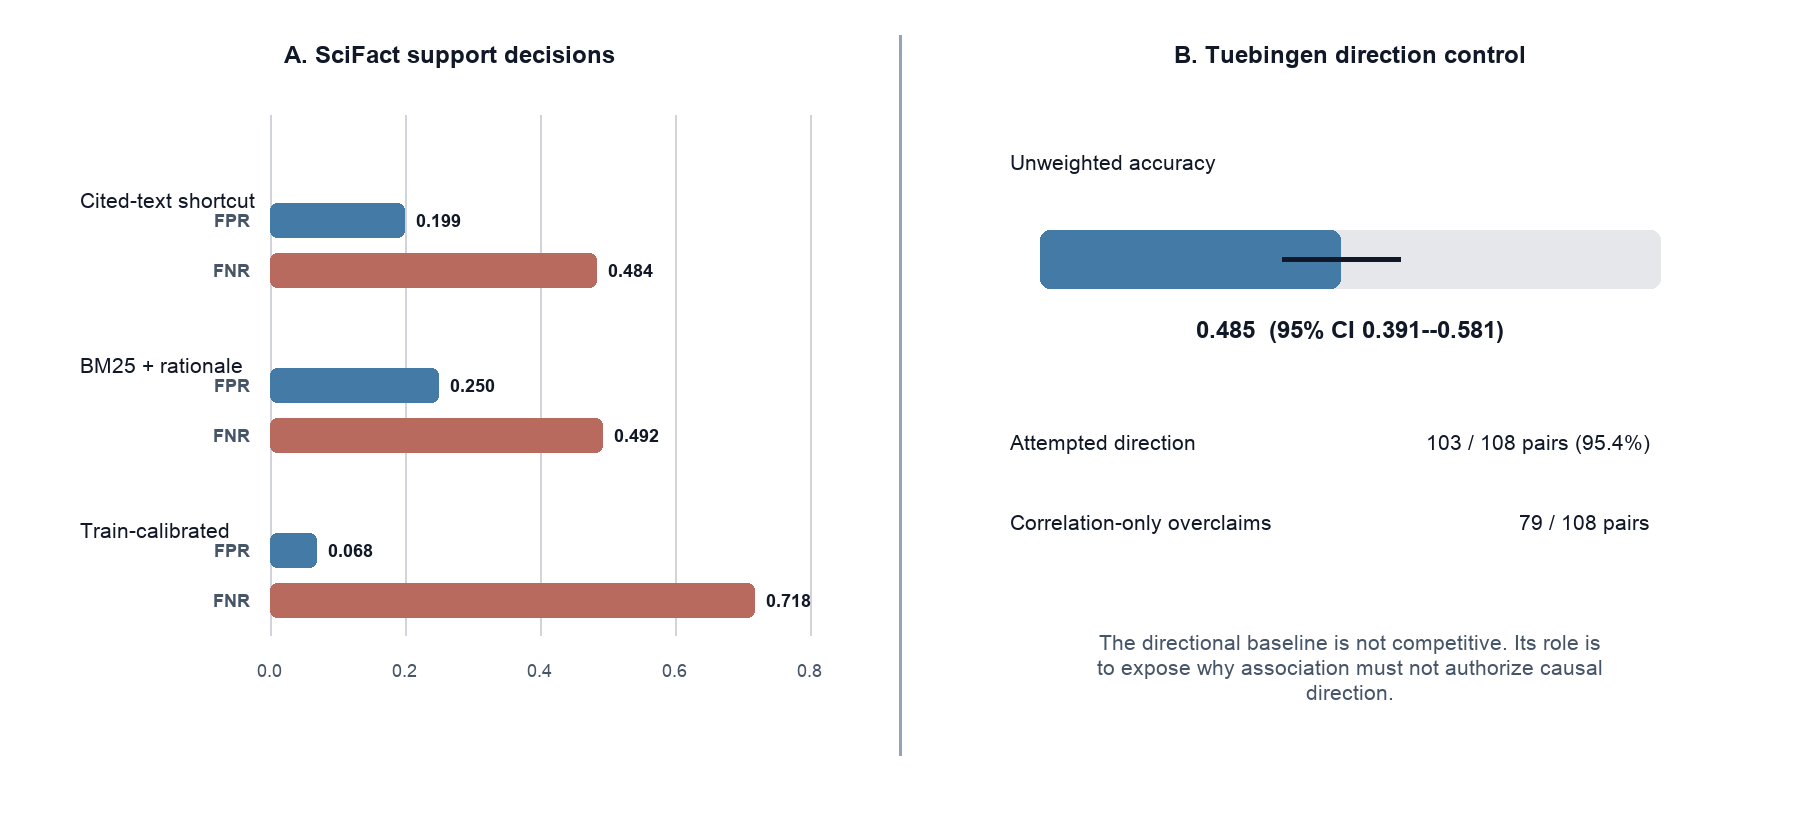
\includegraphics[width=0.96\textwidth]{figures/claimbench_external_controls.png}
\caption{External failure-mode controls. Panel A shows the support-decision
trade-off on the SciFact development split. The calibrated baseline is fitted on
809 training claims and lowers false authorization at the cost of substantially
more false rejection. Panel B reports the bounded Tuebingen directional control.
Its near-chance accuracy blocks any causal-performance interpretation, while 79
strongly associated pairs expose the risk of correlation-only direction claims.}
\label{fig:external-controls}
\end{figure}

\begin{table}[t!]
\centering
\caption{External control results and their admissible interpretation. The controls diagnose overclaiming failure modes and are not presented as competitive task performance.}
\label{tab:external-controls}
\small
\renewcommand{\arraystretch}{1.16}
\begin{tabularx}{\textwidth}{@{}p{0.16\textwidth}p{0.19\textwidth}p{0.27\textwidth}Y@{}}
\toprule
Control & Sample & Principal result & Admissible conclusion \\
\midrule
SciFact & 300 claims & Recall@5 $=0.899$, lexical ORI $=0.199$, BM25-rationale ORI $=0.250$ & Retrieval quality does not authorize support by itself \\
\addlinespace[3pt]
Tuebingen & 108 pairs & 103 attempts, accuracy $=0.485$, 79 correlation-only overclaims & Correlation does not authorize causal direction \\
\addlinespace[3pt]
Known causal graphs & 5 scenarios & Positive and negative controls pass the declared gate & Gate logic handles the tested graph semantics, not causal discovery in general \\
\bottomrule
\end{tabularx}
\end{table}


\section{Regression Ablations and Sensitivity}

The following analyses use the legacy constructed contract cases. They detect implementation regressions and demonstrate which policy components affect the historical decisions. They do not independently validate the scientific taxonomy or calibrate empirical thresholds.

\begin{figure}[t!]
\centering
\resizebox{\textwidth}{!}{%
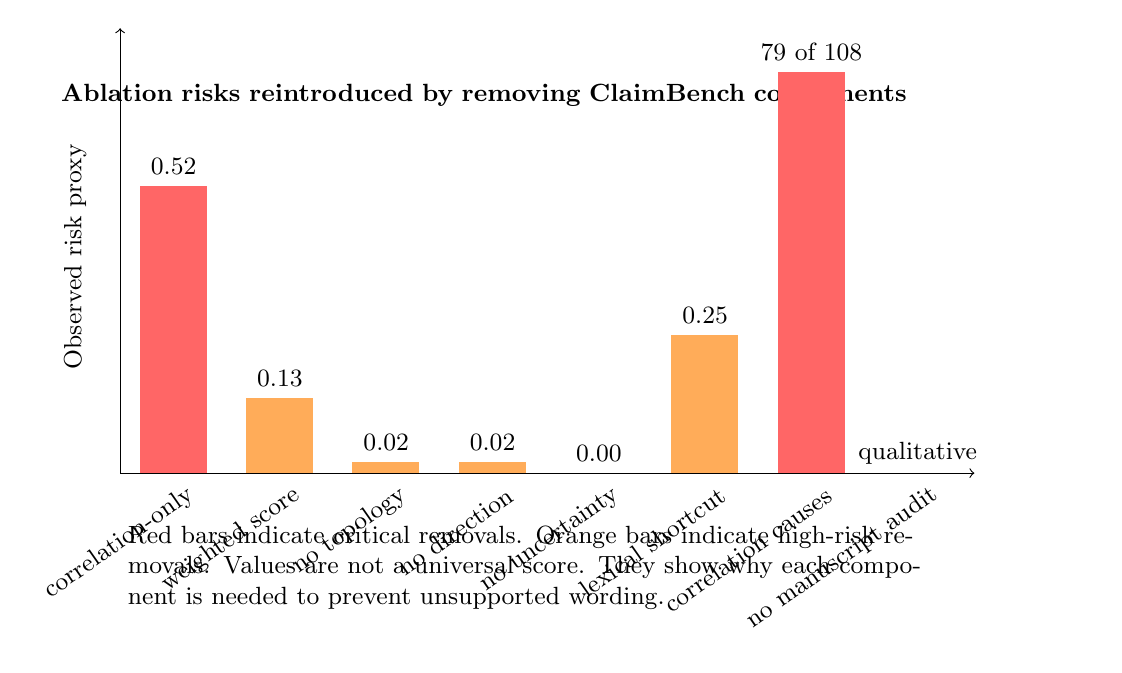
\begin{tikzpicture}[font=\small]
\node[align=left, text width=13cm] at (5.5,4.8) {\textbf{Ablation risks reintroduced by removing ClaimBench components}};
\foreach \x/\h/\lab/\val/\col in {
0/3.65/correlation-only/0.52/red!60,
1.35/0.95/weighted score/0.13/orange!65,
2.7/0.14/no topology/0.02/orange!65,
4.05/0.14/no direction/0.02/orange!65,
5.4/0.0/no uncertainty/0.00/gray!60,
6.75/1.75/lexical shortcut/0.25/orange!65,
8.1/5.1/correlation causes/79 of 108/red!60,
9.45/0.0/no manuscript audit/qualitative/orange!65}
{
  \fill[\col] (\x,0) rectangle +(0.85,\h);
  \node[rotate=35, anchor=east] at (\x+0.75,-0.18) {\lab};
  \node at (\x+0.43,\h+0.25) {\val};
}
\draw[->] (-0.25,0) -- (10.6,0);
\draw[->] (-0.25,0) -- (-0.25,5.65);
\node[rotate=90] at (-0.82,2.75) {Observed risk proxy};
\node[align=left, text width=10.5cm] at (5.1,-1.2) {
Red bars indicate critical removals. Orange bars indicate high-risk removals. Values are not a universal score. They show why each component is needed to prevent unsupported wording.
};
\end{tikzpicture}%
}
\caption{Component ablation summary. Removing non-compensatory gating, causal abstention, or evidence separation reintroduces overclaiming risks that would be hidden by ordinary predictive evaluation.}
\label{fig:ablation}
\end{figure}

\begin{figure}[t!]
\centering
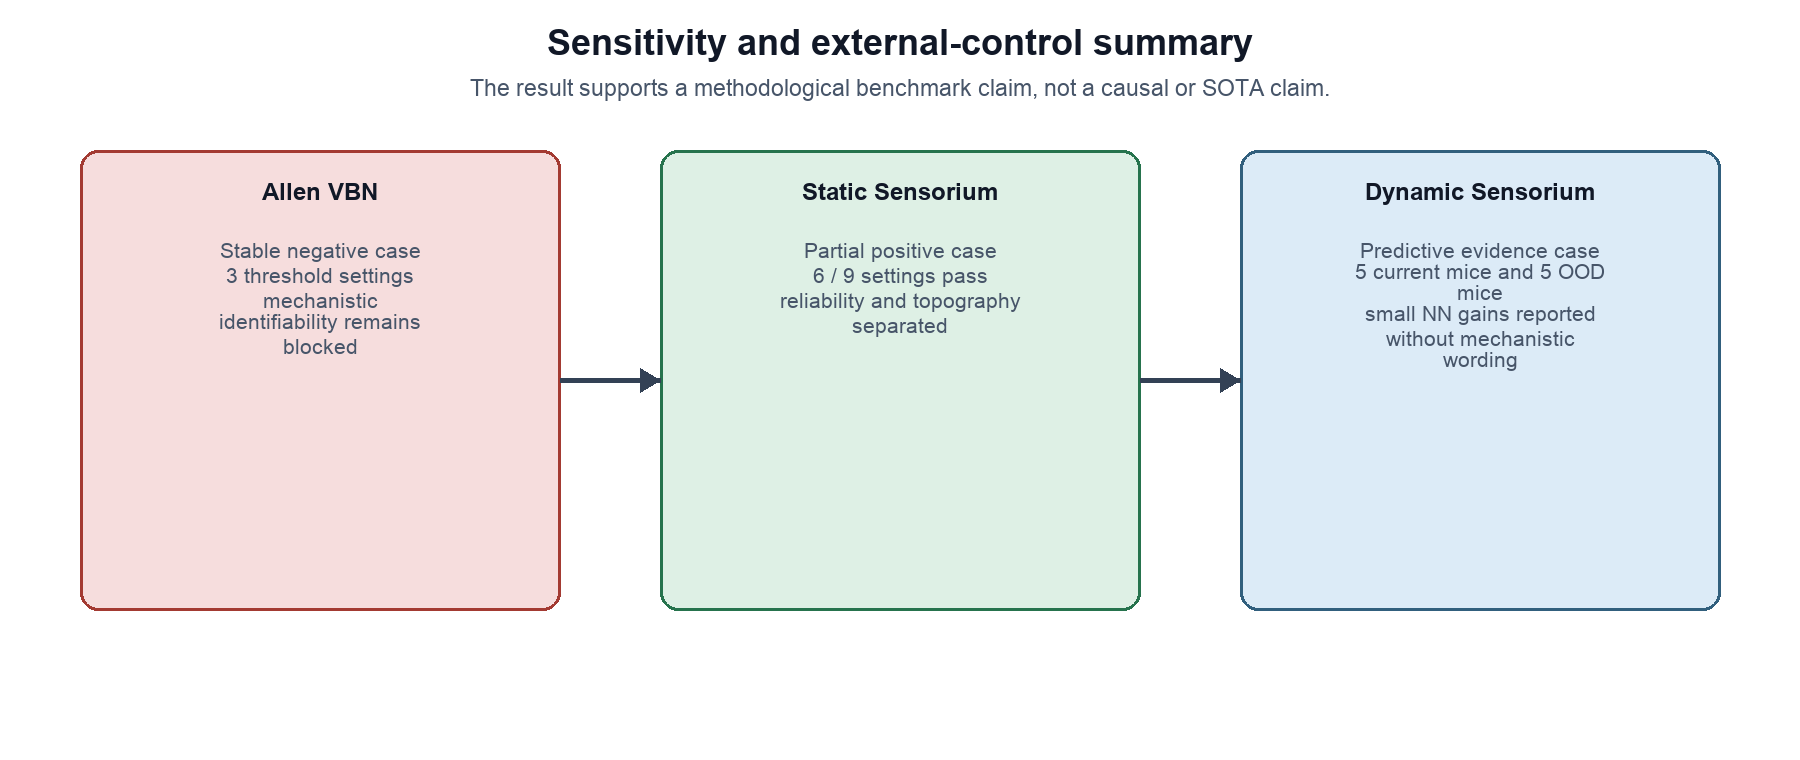
\includegraphics[width=0.94\textwidth]{figures/claimbench_sensitivity.png}
\caption{Sensitivity of the claim gate. Panel A partitions 243 threshold combinations into 108 safe and 135 dangerous cells under the declared criterion. Panel B reports outcomes from deterministic local perturbations of the numerical evidence fields. The resulting stability proportion is an operational robustness measure, not a calibrated probability or confidence interval.}
\label{fig:sensitivity}
\end{figure}


\section{Decision and Release Semantics}

Table~\ref{tab:decision-actions} records the operational consequence of each inference state. Table~\ref{tab:release-summary} records the release checks and the scientific boundaries that remain active after the engineering package passes.

\begin{table}[t]
\centering
\caption{Decision states returned by ClaimBench and their intended editorial consequence. The output is not a ranking of models, but a concrete action on manuscript wording.}
\label{tab:decision-actions}
\small
\begin{tabularx}{\textwidth}{p{0.18\textwidth}p{0.28\textwidth}X}
\toprule
Decision state & Evidence status & Recommended manuscript action \\
\midrule
Supported & All required evidence blocks are present and stable under the declared controls & Keep the claim, but preserve the bounded wording and cite the decision artifact \\
Blocked & At least one non-interchangeable evidence block is missing & Remove the claim or replace it with a weaker statement supported by the available evidence \\
Uncertain & Evidence is present but unstable, threshold-sensitive, or insufficiently confirmed & Report the result as exploratory or requiring confirmation, not as established support \\
Out of scope & The claim family requires evidence not collected by the study & State the limitation explicitly and avoid implying that the framework has evaluated it \\
Needs external review & The decision depends on domain judgement outside the executable artifact & Use the artifact as review support, but keep the final judgement with human experts \\
\bottomrule
\end{tabularx}
\end{table}

\begin{table}[t!]
\centering
\caption{Knowledge-system release generated from clean artifact revisions. Passing checks establish method consistency only. The final four rows remain explicit claim boundaries.}
\label{tab:release-summary}
\footnotesize
\renewcommand{\arraystretch}{1.11}
\begin{tabularx}{\textwidth}{@{}p{0.29\textwidth}p{0.22\textwidth}Y@{}}
\toprule
Check & State & Consequence \\
\midrule
Required KBS artifacts & 9/9 present, expected decisions reproduced, no `-dirty' revision & Method package passes release gate \\
Knowledge profile & Structure, identifier, version, SHA-256 hash, and 22 relation records complete & Inferences bind to an auditable author-proposed policy, not an expert consensus \\
Migration-decision conformance & 40/40 exact matches and 40/40 complete traces & Author-generated migration decisions preserve policy behaviour. They are not external labels \\
Cross-domain empirical generality & Not evaluated & Only the mouse-brain profile is supported empirically \\
External biological replication & Absent & No cross-resource or cross-laboratory replication claim \\
Human outcome effect & Not evaluated and not required by the stated scope & No claim of improved human decisions \\
Complete mouse digital twin & Intervention, whole-brain coverage, entity specificity, independent validation, and operational compute are required & Complete, causal, and entity-specific twin wording blocked \\
\bottomrule
\end{tabularx}
\end{table}


\end{document}
